\section{UPC}
% Overview of UPC
The classic implementation of PGAS is the Unified Parallel C(UPC)\footnote{https://upc.lbl.gov/} language extension from Berkeley. 

\subsection{Overview}
% It was designed to..... for..... used by....

UPC applications, like MPI, follow the Single Program Multiple Data execution model that is explicitly parallel. Defining shared data in UPC can be simply done with the use of the new keyword \verb|shared|. Data declarations without this keyword are inherently private and function as if in a normal non-parallel system. All shared variables may be directly read and written to by any UPC thread, but are physically associated with exactly one of the threads (as shown in Figure \ref{fig:GAS_Diagram}). In the case of arrays, elements can be successively distributed around the network and this distribution schema can be selected by the programmer. 

\begin{figure}[h]
    \centering
    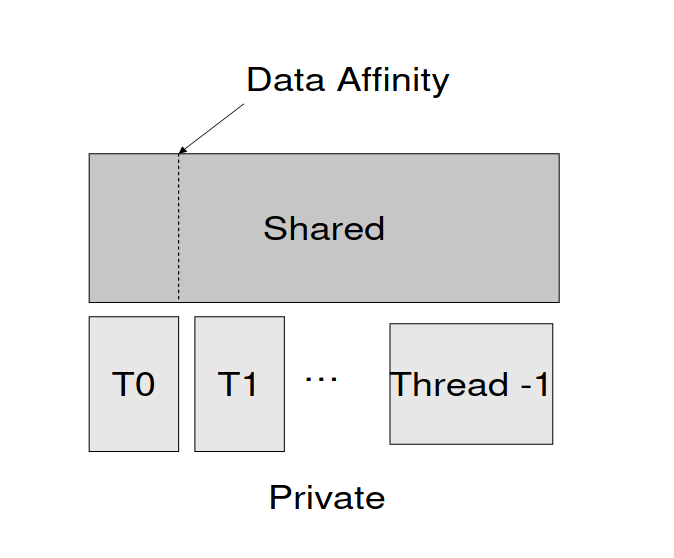
\includegraphics[width=\linewidth]{figures/GAS Diagram.png}
    \caption{UPC Memory Model \cite{UPC_Performance}}
    \label{fig:GAS_Diagram}
\end{figure}

Importantly, UPC provides no memory safety assurances such as mutex locks or semaphores. This avoids adding overhead and implicit synchronisation in the system where it may not be necessary. Therefore, all safety and synchronisation primitives must be implemented by the programmer. UPC provides programmers with full, but arguably unwieldy, control over the data, its storage layout, access patterns, synchronisation requirements and parallelism. With this, performance is highly dependent on the implementation decisions of the programmer. 

UPC's language extension is very minimal on the syntactic level, with all significant changes to the code and logic performed at compile time with the new more involved pointer arithmetic. This is because all references to shared or private data are syntactically identical not only to each other but also to normal C variable accesses - known as implicit data motion. This creates one of the primary pitfalls of UPC. Given the significant inherent disparity in memory access times between local and shared data, it is important that the programmer is explicitly aware of when such shared memory accesses are performed. However, with an implicit memory access model, it is easy for the programmer to mistakenly access shared memory regions in primary compute loops unnecessarily creating significant bottlenecks. However, if written well, performance is expected to be at least parity and often significantly faster than MPI, with an added benefit of \textit{easier} implementation. %but with significant programming ease. 

\subsection{Functionality}
% How it works
Threads are the ``execution vehicle'' for UPC, and do not necessarily correspond with OS threads/processes or a single CPU. Despite this, UPC threads are often implemented as OS-level processes capable of multi-threading processing for greater utilisation of the CPU. In order for these UPC threads to communicate, UPC uses a networking middle-layer application called GASNet. The GASNet communication layer provides very minimal overhead even with a layered network approach and more complex physical address calculations \cite{UPC_Performance}. GASNet includes support for:
\begin{itemize}
    \item RMA 
    \item Active Messages
    \item Various Network APIs including: UDP, TCP/IP, SMP, MPI
    \item NVidia/AMD GPU Memory access
\end{itemize}


% Need references to where this info is from?
Active messages are a form of messaging in which the messages additionally define the necessary handler function they require. This helps to reduce latency and the overheads associated with buffering and provides applications with direct user-level access to network hardware. Each message contains a header with an index to a userspace message handler, so that the contents of the message can be passed to the handler as an argument. This indexing is possible within SPMD execution model as during an initialisation phase each UPC thread is able to register a table that maps indexes to the local virtual addresses of the handler functions. This approach doesn't require address space uniformity between each thread.  